\documentclass[conference]{IEEEtran}

\usepackage{cite}
\usepackage{amsmath,amssymb,amsfonts}
\usepackage{algorithmic}
\usepackage{graphicx}
\usepackage{textcomp}
\usepackage{xcolor}
\def\BibTeX{{\rm B\kern-.05em{\sc i\kern-.025em b}\kern-.08em
    T\kern-.1667em\lower.7ex\hbox{E}\kern-.125emX}}
\begin{document}




\title{Predicting the Stock Market One Quarter at a Time\\
{\footnotesize \textsuperscript{*}Note: Sub-titles are not captured in Xplore and
should not be used}

}

\author{\IEEEauthorblockN{1\textsuperscript{st} Cory Carter}
\IEEEauthorblockA{\textit{Computer Science Master of Science Student} \\
\textit{Oakland University}\\
Auburn Hills, USA \\
email address or ORCID}
\and
\IEEEauthorblockN{2\textsuperscript{nd} Tom Tisdall}
\IEEEauthorblockA{\textit{Software Engineering and IT Master of Science Student} \\
\textit{Oakland University}\\
Auburn Hills, USA \\
ttisdall@oakland.edu}
}

\maketitle



\begin{abstract}
Predicting the stock market is a very challenging task, with hundreds if not thousands of papers addressing this problem.  This paper sets out to explore predictingstock quarterly trends by determining the best quarterly features to use and then leveraging them to determine the direction of the upcoming quarterly report. The thought was to eventually marry this will daily trends to improve accuracy of predicting stock market pricess by factoring in the quarterly direction.  By determining the stocks that will go up or down for a quarter, we will predict whether buying or selling is the best course of action for a stock. Testing for accuracy, we will simuilate buying and selling in the stock market based on our predictions to determine if this project was a succsess or failure.  

**Add more details to this section as we further develop our strategy
\end{abstract}

\begin{IEEEkeywords}
Index Terms - Stock Market, Prediction, Machine Learning
\end{IEEEkeywords}


%Help the reader understand why your research is important and what it is contributing to the field
%Start by giving the reader a brief overview of the current state of research in your subject area.
%Progress to more detailed information on the specific topic of your research.
%End with a description of the exact question or hypothesis that your paper will address.

\section{Introduction}
Determining the direction of a stock from day to day is both a challenging and frustrating problem.  There are so many features to choose from and that factor into a stock changing price from day to day. It can be as simple as positive or negative news, changes in the overall market or industry, technological breakthroughs, production hurdles and many more, which don't even cover the technical or quantative numbers that typically are used to determine a stock rating and predicting its movement from day to day.  This paper is goign to attempt a different tact on predicting stocks, at a more generic and higher level, using the companies quarterly returns.  The thought is this information can be added to other predictors to better refine the accuracy of those models.  In this project we have gathered twenty five Technology, Software and IT Services large and mega cap stocks with earnings history for their entire existence, typically between ten and thirty years.  We started with the features used in the paper Stock Market Trends Prediction after Earning Release  \cite{QuarterlyPrediction}.  We reviewed and refined those quarterly features by using Mutual Info Regression over the datasets that we obtained, which provided us with the most important columns to leverage in our machine learnging algorithm.  We decided to implement Support Vector Machine (SVM) to help us determine what stocks to buy or sell each quarter.  Using our model, we then started with a set amount and bought/sold as recommended to see how we faired in the long run.


\section{Review of existing techniques for predicting the stock market}
For this project, we started by reviewing papers that were published in the realm of stock market analysis via machine learning.  One of the first papers we found Stock Market Analysis: A Review and Taxonomy of Prediction Techniques \cite{TaxonomyofPrediction} discusses how stock market analysis falls into four categories, statistical, pattern recognition, machine learning, and sentiment analysis.  Since this paper focuses on machine learning, we focused on that part of their paper.  They and other papers they referenced felt that the stock market can be predicted, the challenge is determine what information provides the most value in prediction the stock price.  In the paper they discussed they suggest the agorithm space continues to grow with newer techniques like Random Forrest replacing naïve Bayes and  Artificial Neural Networks (ANN), Deep Neural Networks (DNN), and Sentiment Analysis becoming more popular.  They note that in cases where transaction fees are not considered that the traditional models perform better, but where transaction costs are included, the DNN models perform better. Bin, Ahmed and Fadel in their paper Stock Market One-Day Ahead Movement Prediction Using Disparate Data Sources\cite {Onedayahead} that using data from outside the stock market could help improve the prediction accuacy.  In thier paper they proposed using Wikipedia traffic along with stock data helped improve their SVM model.  Using sentiment analysis to predict stock price gains and losses seems to be gaining popularity and some success.  The article Automated Stock Price Prediction Using Machine Learning \cite{AutomatedPrediction} used a SVM with traffic visits to Wiki to determine Apples stock price over time at an 85\% success rate. Unfortunately their prediction testing only used Apple, it woudl have been interesting to see how the model performed against other stocks.  Intestingly enough they did find that the ordering of the features made a difference in their modeling, reminding us that there are many aspects to defining and developing an accurate model.  Automated Stock Price Prediction Using Machine Learning \cite{AutomatedPrediction} also applied sentiment analysis by using news articles to determine positive or negative trends. In their case they found that using a SVM was the best algorithm.  Seeing the benefits of sentiment analysis, this woudl be something we would like to include in future research. 

Changing direction we found other articles that compared recent techniques such as Particle Swarm Optimization, Least Square Support Vector Machine (LS-SVM) and Artificial Neural Network (ANN) to determine which one was a better fit.  A Machine Learning Model For Stock Market Prediction \cite{MLModelPrediction} found that using Particle Swarm to optimize Least Square SVM was better than just LS-SVM by itself and that LS-SVM was better than an Artificial Neural Network (ANN) which tended to run into an overfitting problem. Along the same lines An Emprical Study of Machine Learning Algorithms for Daily Trading Strategy \cite{EmpiricalStudy} compared stocks from the US and Chinese markets across six Machine Learning Algorithms (Logistic Regression (LR), Support Vector Machine (SVM), Classification and Regression Tree (CART) , Random Forest (RF), naïve Bayes (BN) , eXtreme Gradient Boosting (XGB)) and six DNN algorithms (MultiLayer Perception (MLP), Deep Belief Network (DBN), Stacked Autoencoders (SAE), Recurrent Neural Networks (RNN), Long Short-Term Memory (LSTM), Gated Recurrent Unit(GRU)). 

They found that "some traditional ML algorithmshave a better performance than DNN algorithms in most ofthe directional evaluation indicators" and that the best DNN algorithms were not significantly better than the traditional ML algorithms without considering transaction costs.  As transaction costs increase, they found that the ML algorithms performance decreased.  The DNN models degraded when including transaction costs but at a much slower rate than the ML Algorithms.

Interestingly enough, along the same lines of differences in outside variables like transaction costs, Deep Architectures for Long-Term Stock Price Prediction with a Heuristic Based Strategy for Trading Simulations \cite{LongTermPricePrediction} found that when they created an application to simulate trading based on the predictions of their two models Long Short Term Memory (LSTM) and Convolutional Neural Network (CNN) that LSTM outperformed by gaining a higher total dollar amount, but that the CNN model had a higher number of days with gains.  This once again shows that there are many influencers on the stock market that make it challenging to predict.
Predicting the daily return direction of the stock market using hybrid machine learning algorithms \cite {DailyReturnDirection} leveraged 60 financial and economic features showed that using PCA to select features had improved accuracy over those of the entire feature set.  They also found that Deep Neural Networks performed better than Artifical Neural Networks when predicting the stock market.  It is worth noting that most of the papers we researched ended up with prediction models in the range of 55\% to 60\% accuracy which is better than a coin flip but typically not better than the buy and hold strategy.  In summary we found that modeling the stock market is a hard problem with small improvements being the goal and that it is not purely a mathmatelical puzzle to be solved.

\section{Formulation of our solution}
%Method
%A detailed description of the question.
%The methods you used to address the question.
%The definitions of any relevant terminology.
%Any equations that contributed to your work.
In our work we chose to focus on predicting quarterly results, whether the stock would go up or down and by what percent in the next quarter.  For our first step, we gathered quartely data from a site called StockPup.com, which is now defunct. Fortunately we gathered our data before they shut down so we were able to perform our testing with the twenty eight stocks. We chose S\&P 500 large and mega stocks from the technology sector and software \& IT services industry.  The data included fourty one columns to use for predicting.  Before we could use a formula to select the best columns, we had to normalize and clean the data. 
%Cory what steps were used to normalize? Should also talk to newly constructed columns -- for example change over time columns and the window they used.   Talk about generating the class
Once the data was properly cleaned and normalized rather than using all of the features to predict we chose to implement several feature selection algorithms to test with.  This idea came from the paper Predicting the daily return direction of the stock market using hybrid machine learning algorithms \cite{DailyReturnDirection} which found that minimizing the feature set improved the prediction accuracy.  We decided to start by using the Python Library Sklearn with function SelectKBest.  This function provides the abiltiy to choose various algorithms such as f Classification, Mutual Info Classification, Select Percentile and others.  Each of these algoritihms return the top selected features to be used in our model. 

The next step was to classify the data for our model. We implemented a classification category over the average price gain of a stock over several quarters.  The thought was to classifiy the stocks in groups such as those that gained in 1 to 2 percent in a quarter, those that were 2 to 4 percent gains etc. This helped us in a couple of different areas.  First it allowed us to build regression into our calculations by looking at the prior quarters to improve our modeling.  Second we used it in the real world scenario of stock purchasing to decide how risky the stock is. This way we could in the final real world test purchase more of the stocks expected to go up with a bigger gain than the stocks with a minimal gain.  To keep things balanced we opted to always buy some of the positive stocks, trying to eliminate some of the volatility that can come with the higher risk stocks.

After selecting our features we implemented a Support Vector Machine to model and predict our results.  We built our test and train sets of data by selecting a year and quarter to divide the data.  All data prior to the year and quarter chosen was used to train the model. The data from the chosen year and quarter was used to test the accuracy of our model.  We did this rather than splitting the data 80/20 as other processes recommend because we wanted to simulate a real world process.  In the real world we would be predicting the next quarter's price based on the prior quarters.  

After building our model and testing the accuracy, we wanted to prove that our model would be profitable in the real world.  So we started by randomly selecting five stocks to remove from the testing phase and spending \$10,000 to purchase \$2,000 of each stock.  We applied the left over to the cheapest stock to use as much of the \$10,000 as possible. Then we ran our predictions for each quarter to determine if we should buy or sell stock.  To simplify the calculations we rebalanced each quarter, that is sold all of the stock and bought what was recommended by our prediction model.  To validate our project we then compared our process with a buy and hold strategy, which we implemented by purchasing \$2,000 of each stock.


\section{Experimental Results}
Our first step, once we normalized the data was to create a Class that we could use as our target feature.  The class was built as a percent of price change calculated over the prior 3 quarters (we selected 3, but could have used any range). The Class was numbered -1 to 5 based on the percent change from the last few quarters to determine how it was trending.  In our expermiment we wanted to purchase stocks that we predicted had a higher gain likelyhood over those of a lower expected gain.  To do this we broke down the class by percents, 1-2 percent gain would be labeled a 1, 2-3 would be a 2 and so on. This became our target for the feature selection.
In our experiments we felt the most important step would be to properly select the features to include in our model. We tested with several SelectKBest algorithms as you can see in the following images. After several rounds of testing we found that selecting the top 10 features seemed to provide the most consistent and highest accuracy.  We didn't see as much of a change between selecting the proper features that we expected which we attribute to a small data set and many of the columns being directly related to each other.  

Testing with Chi-squared stats of non-negative features (Chi2) \ref{chi2} which we found that it produced an 86\% accuracy.  There were several others that also produced an accuracy of 86\% includeding Mutual Info Regression and F Classification. We saw 87\% with F Classifier (ANOVA F-value), 88\% with Extra Trees Classifier. Our highest accuracy based on feature selection was found when we used Mutual Info Classification \ref{mi}.

\begin{figure}
  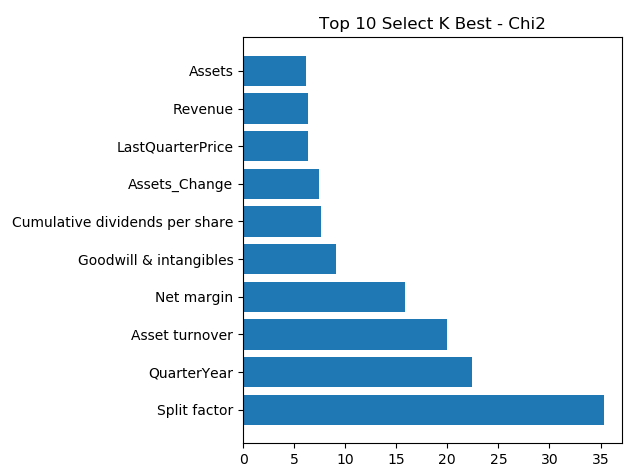
\includegraphics[width=\linewidth]{Top10Chi2.png}
  \caption{Top 10 Chi2 - 86\% Accuracy}
  \label{chi2}
\end{figure}


\begin{figure}
  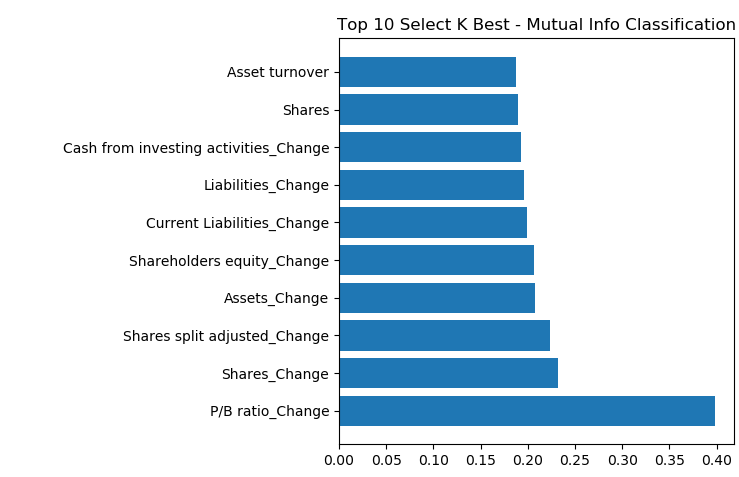
\includegraphics[width=\linewidth]{Top10MutualInfoClassification.png}
  \caption{Top 10 Mutual Info Classification 89\% Accuracy}
  \label{mi}
\end{figure}

Once we completed the target classification and feature selection, we selected to run the experiment with training data from the beginning of each stock through the last quarter of 2016. The test data was selected as 2017 and forward. In our experiment we found the best accuracy with the Mutual Info Classification selecting its top 10 features, completing at an 89\% accuracy rating.  We feel this is much higher than it should be, our thoughts are the limited data set along with an industry that has been growing well over the last several years, is skewing the results to a higher accuracy Interestingly enough, when we selected 5 stocks (EBAY, FB, IBM, NFLX and MA)  to run our cash analysis with the results were less than spectacular.  In fact we found the buy and hold strategy would produce \$17,421.40 where our best strategy using Extra Trees Classifier at 89\% accuracy would only achieve around \$15,400, around \$2,000 less!

%Summarizes your key findings. Include important conclusions that can be drawn and further implications for the field. Discuss benefits or shortcomings of your work and suggest future areas for research.
\section{Summary and Conclusion}

What we learned
--Lot's of features, hard to chose the ones that make a difference
--Outside influences still impact the stock --IE postiive/negative market news, positive/negative industry news, positive/negative company news (for example CEO steps down or is fired etc)
--Importance of feature selection and normalizing the data to compare multiple data sets.


What we could have done better, future improvements
--More data - not enough over time
--looping through the various tests to see how they average out
--


Citations
\begin{itemize}
\item Predicting the daily return direction of the stock market using hybrid machine learning\cite{DailyReturnDirection}
\item Stock Market One-Day Ahead Movement Prediction Using Disparate Data Sources\cite {Onedayahead}
\item Automated Stock Price Prediction using Machine Learning \cite{AutomatedPrediction}
\item Stock Market Analysis: A Review and Taxonomy of Prediction Techniques \cite{TaxonomyofPrediction}
\item International Journal of Computer Science and Telecommunications 4.17-23 \cite {MLModelPrediction}
\item An Empirical Study of Machine Learning Algorithms for Stock Daily Trading Strategy \cite{EmpiricalStudy}
\item Deep architectures for long-term stock price prediction with a heuristic-based strategy for trading simulations \cite{LongTermPricePrediction}
\item How to use Machine Learning to become a millionaire predicting the stock market \cite{WebBecomeMillionaire}
\item I spent 20 minutes trying to predict the stock market with AI, these are my results \cite{20MinStockPredict}
\end{itemize}

\bibliographystyle{IEEEtran}
\bibliography{Bibliography}


\vspace{12pt}


\end{document}
